\section{RT-Pose Dataset} \begin{wrapfigure}{b}{0.5\linewidth}
% \vspace{-20pt}
\centering
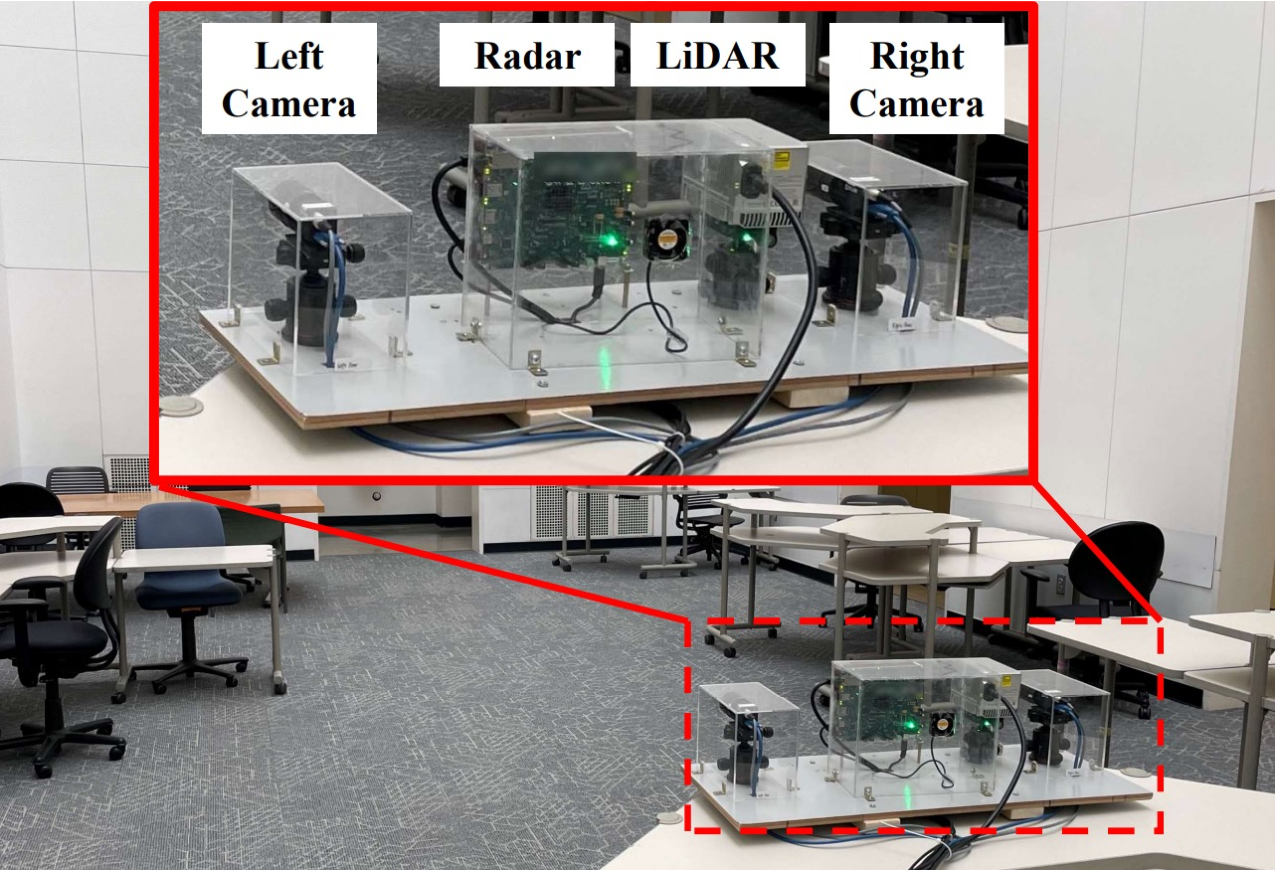
\includegraphics[width=1\linewidth]{fig/device_img.pdf}
\caption{Experimental hardware setup in an indoor environment for data collection.}
\label{fig:device}
% \vspace{-20pt}
\end{wrapfigure}
To construct the dataset, we recruit 10 participants to perform 6 types of actions. The experiments are divided into two categories. In the first category, participants are required to perform actions while standing, including waving, lifting legs, and random poses to increase the complexity of the actions. A video sequence of random poses involves a subject randomly performing one possible movement at a time, including stretching, bending, twisting, etc., each lasting 3 to 5 seconds. The second category focuses on walking, with additional actions added during the process, such as walking and waving or sitting down after walking. Each type of action is inherited from previous radar-based datasets \cite{xue2021mmmesh,sengupta2022mmpose,an2021mars}. Each sequence contains one action for 30 seconds, providing a variety of different difficulty levels. 
As a result, people can thoroughly evaluate their 3D HPE methods on a broad distribution of actions with diverse difficulties. 
Furthermore, we provide the dataset development kit to facilitate the usage and evaluation of future methods.
\begin{figure}[t]
\centering
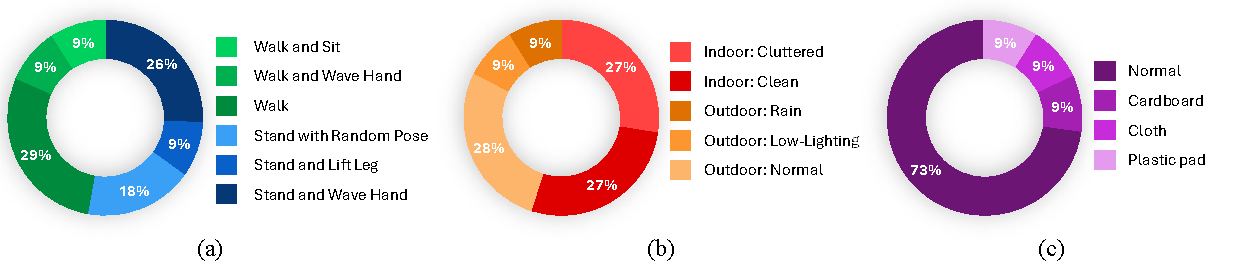
\includegraphics[width=1\linewidth]{fig/data_distribution_img.pdf}
\caption{Data distribution for RT-Pose dataset: (a) Activities; (b) Environmental conditions; (c) Occlusion conditions}
\label{fig:data_distribution}
% \vspace{-20pt}
\end{figure}

\subsection{Sensors}
The data collection hardware system comprises two RGB cameras, a non-repetitive horizontal scanning LiDAR, and a cascade imaging radar module, as shown in Figure~\ref{fig:device}. 
To extract human pose information from radar signals, the radar module's parameters have been specifically configured.
The radar operates at ten frames per second in this work. The radar module is equipped with 12 transmit (TX) and 16 receive (RX) antenna elements and operates in a multiple-input multiple-output (MIMO) mode~\cite{kim2021human}. 
This radar module provides the azimuth and elevation angle resolutions of 1.4 degrees and 18 degrees, respectively. Furthermore, this work implements a high-frequency slope with a long ramp time to efficiently utilize the hardware's sweep bandwidth, ranging from 77 GHz to almost 81 GHz. The longer sweep bandwidth of a chirp increases the radar range resolution~\cite{klauder1960theory,sengupta2020mm}, which is 4.5 cm in this work. Each frame consists of 64 chirps used for calculating radar Doppler signals, providing a velocity resolution of 3.9 cm/s. These carefully chosen configurations ensure the system's accuracy and reliability in capturing human poses.



\subsection{Data Collection}
We collect the dataset in 40 scenes with indoor and outdoor environments. 
Figure~\ref{fig:env} shows some of the collected data.
Indoor environments include clean and cluttered conditions, while outdoor ones include normal, rainy weather, and low-lighting conditions. Each experimental condition includes 8 scenarios, which are nonocclusive, and three occlusive conditions (cardboard, cloth, and plastic pad). 
Each nonocclusive and occlusive condition is recorded in single- and multi-person settings.
To consider the different fields of view (FoV) of all sensors, the sensor suite is situated 109 cm above ground, and an appropriate detection area is planned based on different scenarios. 
\begin{figure}[t]
\centering
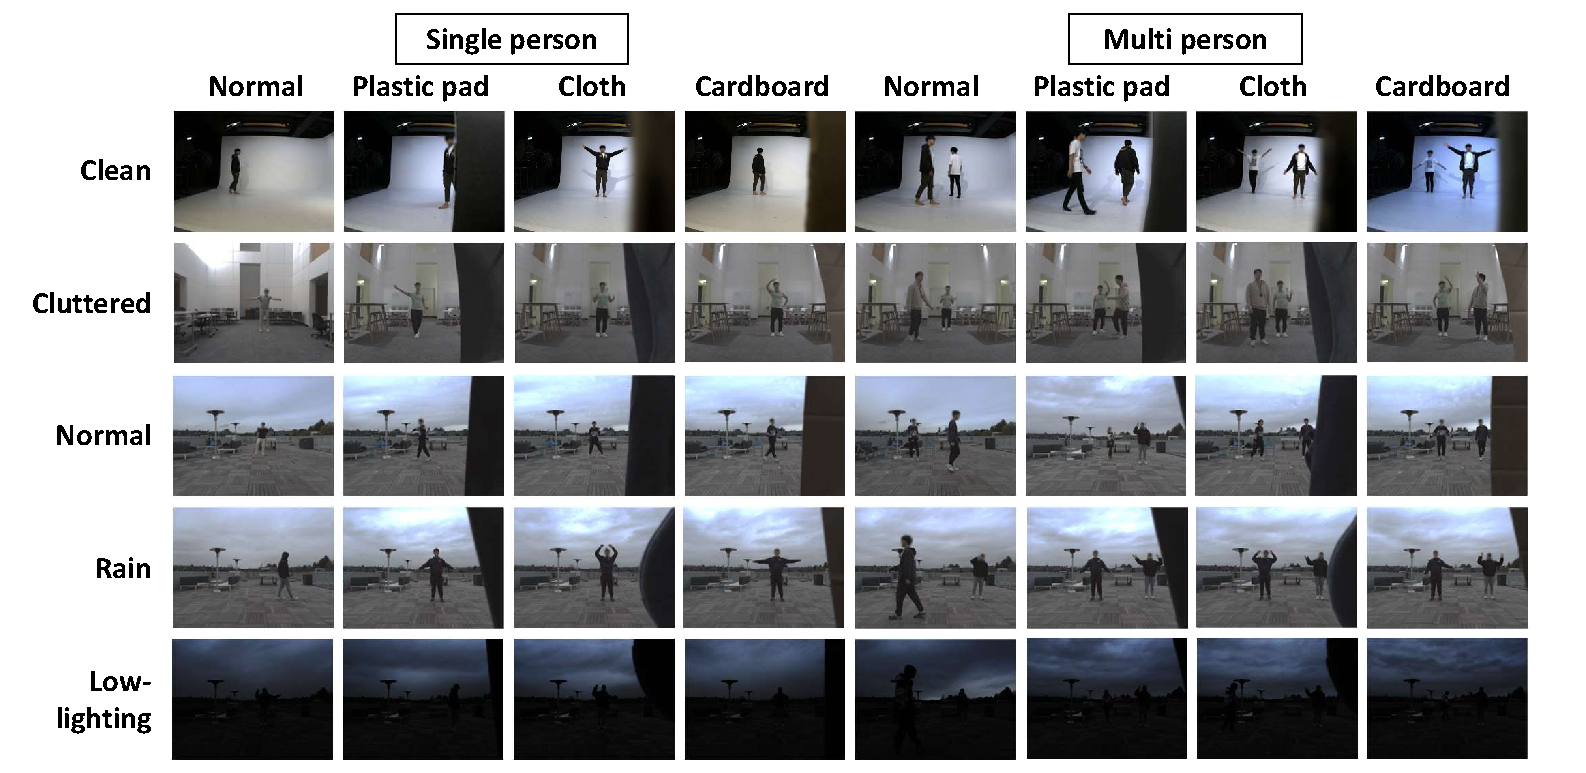
\includegraphics[width=0.9\linewidth]{fig/env_img.pdf}
\caption{Experimental instances across various indoor and outdoor conditions with diverse scenarios for data collection.}
\label{fig:env}
\end{figure}
\subsection{Data Processing}
\begin{figure}[t]
    \centering
    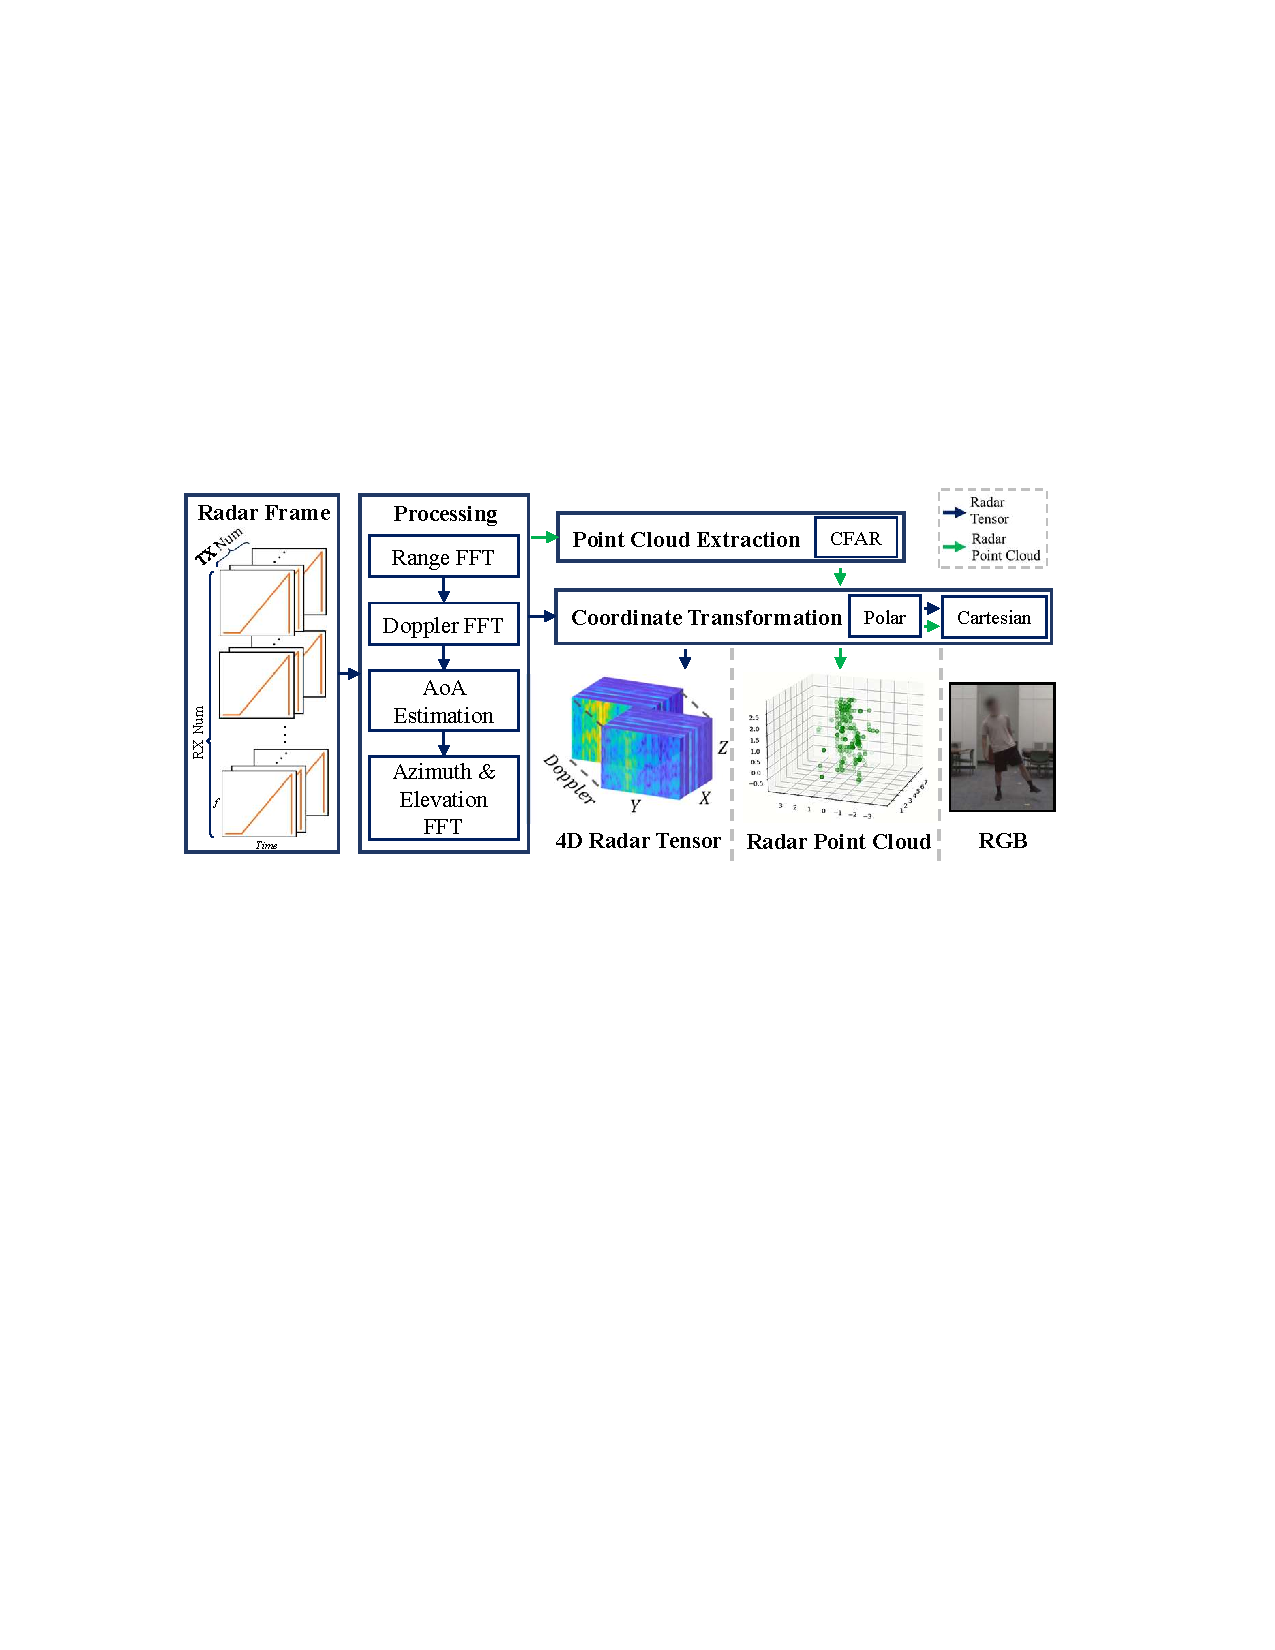
\includegraphics[width=0.75\linewidth]{fig/radar_process.pdf}
    \caption{Radar signal processing flow. The green arrow line is for radar point cloud generation and the blue line is for 4D radar tensor generation. }
    \label{fig:radar_process}
\end{figure}
The captured radar signal, referred to as 4D tensor data, is processed by a series of steps \cite{heath2016overview, neemat2019reconfigurable, cruw3d}, as shown in Figure~\ref{fig:radar_process}. 
On the transmitter side, the frequency of the transmitted signals, or chirps, periodically increases based on the set frequency slope. 
Consequently, the received signal exhibits a different frequency than the transmitted signal. 
The frequency difference between transmitted and received signals can be used to estimate the range of the object reflecting the signal to the radar sensor by the Fast Fourier Transform (FFT). 
At the beginning of the data processing, each radar frame consists of 64 chirps, resulting in 64 range estimation results. Utilizing this range information, the velocity of the responding object can be measured through FFT, a phenomenon known as the Doppler effect. 
Second, the radar signal data is re-modulated according to the antenna position. This step is essential for the calculation of the angle of arrival (AoA), enabling the generation of highangular resolution results. 
Third, the radar signal from the azimuth and elevation directions also undergoes FFT processing to represent velocity responses in different directions. Finally, the entire radar data is transformed from polar coordinates to Cartesian coordinates. This transformation enhances the intuitiveness for the subsequent pose estimation. In this study, the processed 4D radar tensor has the dimension of $64\times32\times128\times256$, which correspond to velocity, the $z$-axis, the $y$-axis, and the $x$-axis, respectively.

\subsection{Annotation Workflow}

\begin{figure*}[t]
\centering
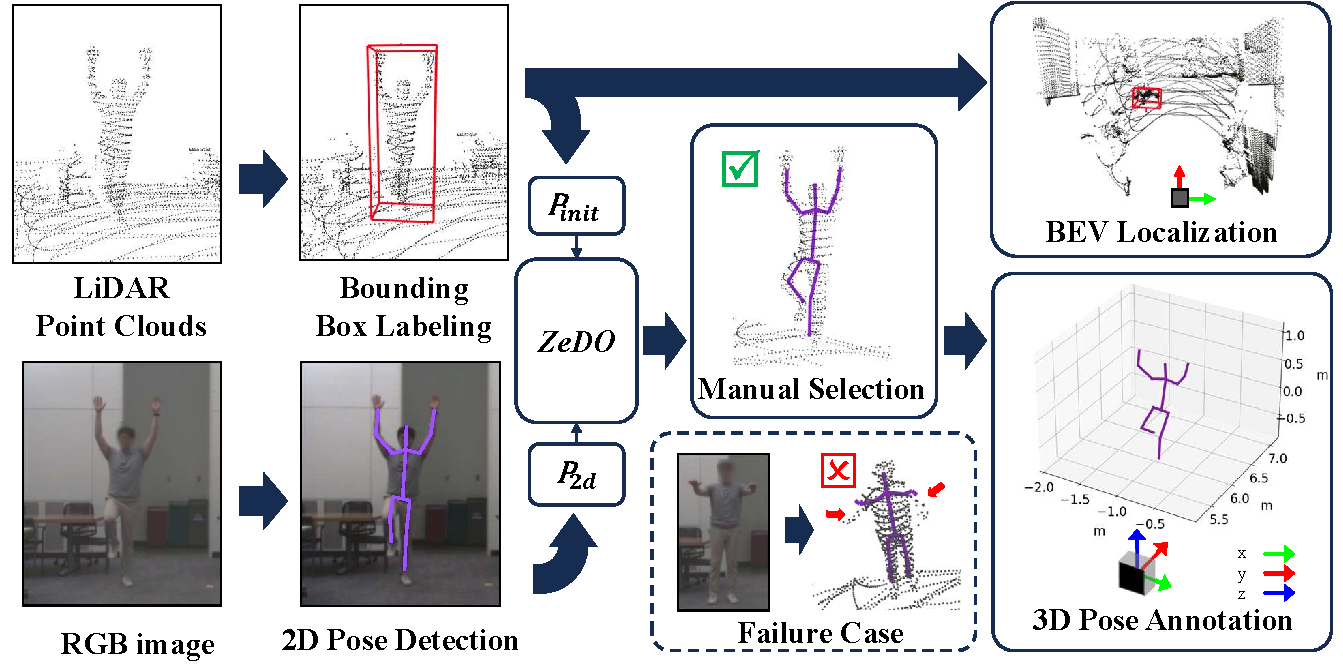
\includegraphics[width=0.75\linewidth]{fig/Annotation_flow.pdf}
\caption{Workflow of human localization and 3D pose ground truth annotations. Estimated 2D pose results, predicted by the pre-trained HRNet model, are denoted as \(P_{2d}\). The initial setting pose derived from LiDAR point clouds is denoted as \(P_{init}\). Both \(P_{2d}\) and \(P_{init}\) are inputs into ZeDO, an optimization-based pipeline for 3D pose estimation.}
\label{fig:annotation}
% \vspace{-20pt}
\end{figure*}
To achieve accurate human subject detection in a larger area with high-quality ground truth, our system integrates LiDAR and RGB camera data, as illustrated in Figure~\ref{fig:annotation}. The images provided by the camera are processed using the HRNet~\cite{sun2019deep} to extract 2D human poses. Then, a 3D HPE model, called ZeDO~\cite{jiang2024back}, utilizes the 2D poses to estimate the 3D poses as the initial 3D pseudo ground truth. However, estimating 3D poses using a monocular camera often lacks precision and stability in depth. Therefore, this work incorporates LiDAR for depth estimation of the human subject center. The LiDAR sensor captures environmental information and the subject's point cloud data, ensuring errors are under 2 cm inside the detection range of 20 m. The human subject is manually labeled with a 3D bounding box, which can provide an accurate 3D position.

ZeDO, a state-of-the-art (SOTA) method for cross-dataset HPE, implements an optimization-based pipeline for 3D pose estimation using 2D poses. This method requires 2D poses as input, and ZeDO is able to estimate multiple-hypothesis 3D poses. In this research, the center of the 3D bounding box provided by LiDAR is utilized as the pelvis of the initial pose, which enhances the accuracy of depth estimation compared to relying solely on the monocular camera data, and improves the performance of ZeDO. With the imported 2D pose from HRNet~\cite{hrnet}, ZeDO iteratively refines the 3D poses. To further improve annotation accuracy, an annotation tool is developed for manual selection and optimization of each frame to retain correct 3D human poses. The 3D HPE results from ZeDO will be put in the LiDAR point cloud for visualization, which is beneficial for humans to filter and modify the error pose annotation results. About 30\% of the data is removed or optimized after human correction, and this process ensures the quality of keypoints annotation. More details can be found in the supplementary material.







